\chapter{INTRODUCTION}
\section{Background}
\label{ch:background}
In this day and age, Exploration of space has been one of the driving force for technological innovation, pushing the boundaries on what is possible in the human. Theres a challenge in space exploration is the safe return of spacecraft and payloads to Earth or other celestial bodies with an atmosphere. During atmospheric reentry, a vehicle traveling at hypersonic speeds experiences extreme aerodynamic heating, which can lead to catastrophic failure if not properly managed. To protect the vehicle from these extreme temperatures, a thermal protection system (TPS) is required.
\par
For generations, Rigid-like TPS that have been the standard solution for atmospheric earth reentry such as Reusable TPS, Structuraly Integrated TPS, Hot Stracture, and Ablator~\cite{TPS-stateofIndustryNASA}. However, the size of a rigid heat shield is limited by the launch vehicle's payload fairing, which in turn restricts the size and mass of the reentry vehicle. This limitation poses a challenge for future missions that require the landing of large payloads and it's flexibility on it's backups, such as human missions to Mars or the return of large assets from space.


\par
To conterr-act this challenge, an deployable entry systems called inflatable aerodynamic decelerators (IADs) TPS has been emerged and tested as a non integrated TPS and flexible \cite{DiNonnoLOFTID}. IADs, also known as hypersonic inflatable aerodynamic decelerators (HIADs), are lightweight, flexible structures that can be packed into a small volume during launch and then inflated to a much larger size before atmospheric entry. The large surface area of an IAD provides significant aerodynamic drag, allowing for the deceleration of large masses at higher altitudes where the air is less dense and the heating is less severe.
\begin{figure}[H]
    \centering
    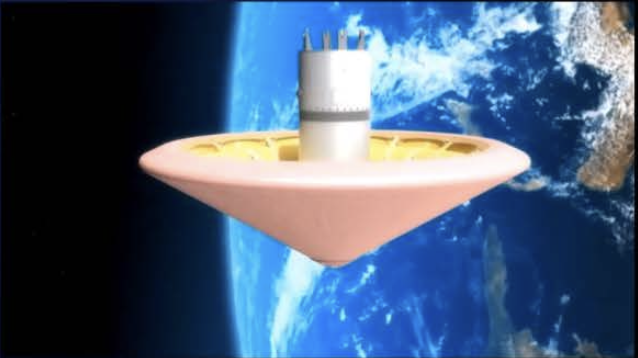
\includegraphics[width=0.5\textwidth]{gambar/HIADsDeployed.png}
    \caption{HIADs when deployed}
    \label{fig:Hiaddeployed}
\end{figure}

\par
The development of IADs approach that combines aerodynamics, structural mechanics, and materials science. A key component of an IAD is the flexible thermal protection system (FTPS), which is responsible for protecting the inflatable structure from the intense heat of reentry. The FTPS is a multi-layered system that typically consists of an outer fabric, insulation layers, and a gas barrier \cite{Guo2011Polyimide}. The design and analysis of the FTPS task that requires accurate modeling of the aerothermal loads and the material response.

\begin{figure}[H]
    \centering
    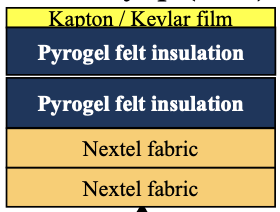
\includegraphics[width=0.5\textwidth]{gambar/IADsLayer.png}
    \caption{IADs Layer Example}
    \label{fig:Hiaddeployed}
\end{figure}

\section{Problem Statement}
The successful design and operation of an IAD depend on the ability to accurately predict and manage the unusual edge aerothermodynamic environment and the complex fluid-structure interaction (FSI) phenomena that occur during atmospheric reentry. The flexibility of the IAD structure and the FTPS adds a layer of complexity to the analysis that is not present in traditional rigid heat shields (Missing Citation). The deformation of the IAD under aerodynamic loads can affect the flow field and the heat transfer to the vehicle, which in turn can affect the structural response.

Therefore, there is a critical need for numerical tools and methodologies to model the coupled FSI and aerothermal behavior of IADs. These tools must be able to capture the complex physics of hypersonic flows, including real gas effects, chemical reactions, and turbulence. They must also be able to model the nonlinear structural response of the inflatable structure and the thermal response of the FTPS.

\section{Research Objective}
In this research of this thesis, the objectives is to develop and to study a computational fluid dynamics (CFD)-based methodology for the aerothermal and aerodynamic analysis of a flexible thermal protection system for an inflatable aerodynamic decelerator (IAD). The study will focus on adapting and applying the methodology presented in the work of Al-Obaidi et al. \cite{AlObaidi2021Parametric} to the specific case of an IAD.

The specific objectives are:
\begin{enumerate}
    \item \textbf{Geometric Modeling:} To generate 2D axisymmetric CFD models of a Hypersonic Inflatable Aerodynamic Decelerator (HIAD) based on IRVE-3 specifications, specifically contrasting the \textit{scalloped} surface topology/geometry of stacked toroids against an equivalent \textit{smooth} rigid sphere-cone baseline.

    \item \textbf{Flow Field Geometrical Model Analysis:} To analyze the impact of surface waviness on the hypersonic shock structure, specifically quantifying the \textit{bow shock standoff distance} ($\Delta$) and identifying the presence and stability of \textit{recirculation zones} (vortices) within the gaps (valleys) of the inflatable rings.

    \item \textbf{Aerothermal Load Analysis:} To determine and compare the surface distributions of \textit{Wall Heat Flux} ($q_w$) and \textit{Wall Shear Stress} ($\tau_w$), with a focus on identifying peak heating augmentation at the toroidal crests versus heat flux alleviation in the valleys compared to the smooth baseline.

    \item \textbf{Aerodynamic Performance Evaluation:} To calculate and compare the integral aerodynamic forces, specifically the \textit{Drag Coefficient} ($C_d$), to determine if the scalloped geometry provides a deceleration advantage over the rigid baseline.
\end{enumerate}

\section{Research Gap}
Based on the literature reviews, we identify several gap from the available data of this design.
\textit{It will be further elaborated on Chapter IV and Chapter V}
\begin{itemize}
    \item \textbf{High-Resolution Surface Mapping:} Resolving the heat flux and pressure distribution along the "scalloped" wetted length to quantify the heating penalty factor.
    \item \textbf{FTPS Safety Margin Analysis:} Determining the quantitative gap between predicted peak heating and the $103 \text{ W/cm}^2$ limit of Gen-2 SiC materials under scalloped flow conditions.
\end{itemize}

\section{Scope and Limitations}

The scope of this research is strictly defined to provide aerothermal and aerodynamic analysis of the Flexible Thermal Protection System (FTPS) within the constraints of available computational resources. The boundaries and limitations of this study are as follows:

\begin{enumerate}
    \item \textbf{Geometric Representation:} The HIAD structure is simplified by assuming a fully inflated and rigid shape. While the actual inflatable decelerator is flexible, this study treats the "scalloped" toroidal stack as a non-deformable geometry to isolate the impact of surface topology on the flow field.
    
    \item \textbf{Dimensionality:} The investigation is restricted to a \textbf{2D Axisymmetric} model. This approach assumes a zero angle of attack ($\alpha = 0^\circ$) to maintain rotational symmetry, allowing for higher grid resolution in the boundary layer while remaining within hardware memory (RAM) limits.
    
    \item \textbf{Numerical Framework:} The fluid flow is governed by the \textit{Reynolds-Averaged Navier-Stokes} (RANS) equations. The simulations are executed using the \textit{Density-Based Coupled Solver} within the ANSYS Fluent commercial numerical suite, utilizing a second-order upwind discretization scheme for shock capturing.
    
    \item \textbf{Turbulence Modeling:} The \textit{Shear Stress Transport} (SST) $k-\omega$ model is employed to resolve the turbulence. This model is specifically selected for its superior ability to handle flow separation and recirculation zones within the toroidal valleys.
    
    \item \textbf{Thermophysical Gas Model:} To account for the extreme hypersonic conditions, \textit{real gas effects} are incorporated through a \textbf{Thermally Perfect Gas} model, which accounts for the temperature-dependency of specific heats ($C_p$). 
    
    \item \textbf{Chemical Modeling:} Although the flow is hypersonic, chemical dissociation is handled through a simplified approach. While the high-enthalpy effects are acknowledged, the gas is assumed to be in \textit{chemical equilibrium} or frozen, neglecting finite-rate non-equilibrium chemical reactions. This limitation is necessary to ensure solver stability and computational efficiency on standard workstation hardware.
\end{enumerate}

\section{Methodology Overview}
This study approach using simulation-based to analyze the aerothermal performance of surface topology/geometry on a Hypersonic Inflatable Aerodynamic Decelerator (HIAD). The data used in this study is derived from parametric geometric modeling then resolving flow gradients such as shock waves and boundary layers. From this analysis, the scalloped (inflatable) geometry is compared against a smooth (rigid) baseline to evaluate its thermal mitigation potential. The study begins with a comprehensive literature review and concludes with an estimation of aerodynamic heating reduction, as illustrated in Figure \ref{fig:flowchart_ch1}. The research stages are structured sequentially as follows:

\begin{figure}[h]
    \centering
    % Placeholder for the flowchart image
    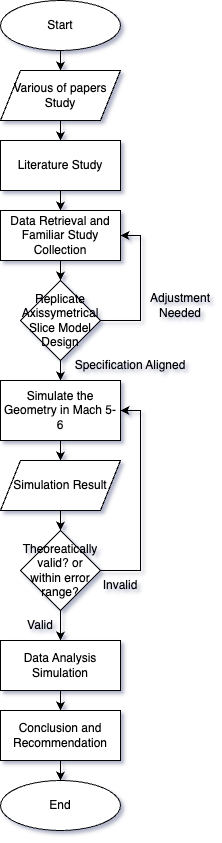
\includegraphics[width=0.21\textwidth]{gambar/flowchart.png}
    \caption{Research Methodology Flowchart.}
    \label{fig:flowchart_ch1}
\end{figure}

\subsection*{a. Literature Study}
The initial stage of the study is conducting literature study. In this phase, the researcher reviews various references related to the concept of Hypersonic Aerothermodynamics, the physics of shock-boundary layer interaction, the implementation of turbulence modeling (SST $k-\omega$), and the formulation of Thermally Perfect Gas models. This literature review is conducted to obtain a strong theoretical foundation for designing the computational domain, determining the critical flow parameters ($Ma$, $Re$, $T$), and supporting the analysis and simulation stages.

\subsection*{b. Geometric Modeling and Data Generation}
Research data is obtained from parametric geometric modeling generated via Python scripting within the FreeCAD environment. This data contains the coordinate definitions of the vehicle profiles, specifically the toroidal radii and valley depths for the "scalloped" configuration and the tangent-cone angle for the "smooth" baseline. These geometric parameters serve as the primary input for the discretization process.

\subsection*{c. Numerical Simulation and Processing}
This stage encompasses several key computational steps. First, the geometric data is discretized into a hybrid mesh with strict near-wall refinement ($y^+ \approx 1$) to resolve the viscous sublayer. Next, the physical models are configured within the Density-Based Coupled Solver, specifically enabling the Equation of State for compressible flow and Sutherland’s Law for viscosity.

The simulation process aims to resolve the flow field around the vehicle to identify regions of peak heating and flow separation. The meshed geometries are subjected to hypersonic freestream conditions ($Ma > 5$) to represent the re-entry environment. The simulation is conducted using a steady-state approach to determine the converged values of heat flux and drag.

The initial simulation results are validated against theoretical correlations. If significant discrepancies are found (e.g., residuals not converging or physical instability), the grid parameters are refined, and the simulation is repeated until the solution achieves statistical stationarity. Thus, the simulation not only yields flow visualization but also ensures the numerical validity of the aerothermal predictions.

\subsection*{d. Data Analysis}
In this stage, the simulation results are analyzed to evaluate the thermal efficiency of the proposed geometry. The analysis is performed by comparing two main scenarios: the scalloped inflatable profile and the smooth rigid baseline. The parameters compared include the Stagnation Point Heat Flux, the Wall Heat Flux distribution along the flank, and the total Drag Coefficient ($C_d$). The results are then used to calculate the percentage reduction in peak heating and to identify any local hot spots caused by shock impingement in the valleys.

\subsection*{e. Conclusion and Recommendations}
The final stage of the research is the current conclusions and what comes next. Based on the analysis results, the thermal performance of the scalloped geometry is determined relative to the baseline. This research also presents recommendations regarding the optimal geometric configuration (toroid radius vs. gap size) as an empirical basis to support the design of future   systems. Recommendations are addressed to future researchers and aerospace engineers as a basis for decision-making in the effort to improve the efficiency and thermal safety of atmospheric re-entry vehicles.

\section{Thesis Outline}
The  structure of this thesis arranged as such. A brief description of each chapter is outlined as follows:

\textbf{CHAPTER I} This chapter contains the research background, problem statement, research objectives, scope of study, methodology overview, and the systematic thesis outline. This section is providing an initial overview regarding the rationale for conducting the research, the specific goals to be achieved, and the limitation of the research scope, and established the writing framework/systematic plan.

\textbf{CHAPTER II} This chapter contains the theoretical framework and literature review that supports this. It discusses the fundamental concepts of Hypersonic Aerothermodynamics, the physics of Shock-Boundary Layer Interaction (SBLI), the formulation of the Shear Stress Transport (SST) turbulence model, and the thermodynamic properties of high-temperature gases (Thermally Perfect Gas). This chapter also reviews relevant previous studies to establish the state-of-the-art.

\textbf{CHAPTER III} This chapter contains the research schedule plan, covering the sequential stages of the investigation. This includes the parametric geometric modeling in FreeCAD, the computational domain discretization (meshing strategy), the numerical configuration of the density-based CFD solver, and the validation procedures. It describes the complete workflow of the research execution from the initial design to the final simulation.

\textbf{CHAPTER IV} This chapter contains the theoretical hypothesis and predicted aerothermal phenomena based on the literature study. Instead of final simulation results, this chapter synthesizes existing research to predict/forecast the expected result characteristics, such as shock wave structures and recirculation regions in the scalloped valleys. It establishes the performance expectations and physical hypotheses that will be subsequently verified during the simulation phase.

\textbf{CHAPTER V} contains the summary of the research findings derived from the data analysis in the previous chapter. This section presents the final conclusions regarding the aerothermal performance of the scalloped HIAD and provides recommendations for future researchers and aerospace engineers as a basis for further development in hypersonic deceleration systems.